%%%%%%%%%%%%%%%%%%%%%%%%%%%%%%%%%%%%%%%%
%%  JOE B. https://github.com/joebd %%%%
%%%% POLS 702 REPLICATION %%%%%%%%%%%%%%
%%%%%    PRESENTATION     %%%%%%%%%%%%%%
%%%%%%%%%%%%%%%%%%%%%%%%%%%%%%%%%%%%%%%%
%%%%%%%%%%%%%%%%%%%%%%%%%%%%%%%%%%%%%%%%
%%%%%%%%%%%%%%%%%%%%%%%%%%%%%%%%%%%%%%%%
\documentclass{beamer}
\usetheme{cambridgeus}
\usepackage{amsmath}
\usepackage{amsthm}
\usepackage{relsize}
\usepackage{dcolumn}
\usepackage{dcolumn}
\usepackage{booktabs}
\newtheorem*{h1}{(H_1)}
\setbeamertemplate{footline}[frame number]{} % Shows # of slides in corner 
\setbeamertemplate{navigation symbols}{}
\setbeamertemplate{footline} [frame number]{}

\title{Political Party Competition and Campaign Finance Laws}
\author{Joe B. - https://github.com/joebd}

\begin{document}

% TITLE 

\begin{frame}
\maketitle
\end{frame}
	
% OVERVIEW

\begin{frame}
	\frametitle{Overview}
	\begin{itemize} 
		\item{Background} \\~\
		\item{Synopsis} \\~\
		\item{Replication Methodology} \\~\
		\item{Research Proposal} \\~\   
	\end{itemize}
\end{frame}


%% INTRODUCTION

\begin{frame}{title}{Does campaign finance laws influence political party competition?}
	\frametitle{Introduction} 
Potter, Joshua D. and Margit Tavits. 2015. "The Impact of Campaign Finance Laws on Party Competition." \emph{British Journal of Political Science} 45(1): 73-95. \\~\
\begin{itemize}
		\item{Comparative Perspective} \\~\
		\item{Democratic elections} \\~\
		\item{Campaign Finance} \\~\
\end{itemize}
\end{frame}

%% SYNOPSIS 

\begin{frame} 
	\frametitle{Synopsis}
Test the relationship of campaign finance laws and political party competition. \\
\vspace{1cm}
Development of an independent variable \underline{fund parity}, which captures the campaign finance laws in each democratic country.  
\end{frame}

% HYPOTHESIS
		%% Also adding the OLS results and a plot of the countries 
		% After this slide ^ 
	
\begin{frame}
	\frametitle{Hypothesis}
	\begin{block}{}
		\textbf{{H1})}: \emph{Where fund parity is high, more fractionalized party systems with a higher effective number of parties}
	\end{block}
\end{frame}

%% REPLICATION METHODOLOGY

\begin{frame}
		\frametitle{Replication Methodology}
		\centering
		\textbf{Regression Analysis (OLS)} \\
\end{frame}

% OLS Model Estimates Table 

\begin{frame}
	\frametitle{\emph{OLS Model Estimates (Potter and Tavits 2015)}}
	\begin{table}
		\centering 
		%  \label{} 
		\small
		\begin{tabular}{@{}lD{.}{.}{-3} D{.}{.}{-3}@{}} 
			\toprule
			& \multicolumn{1}{c}{All democracies} & \multicolumn{1}{c}{1974 and later}\\ 
			\midrule
			Fund Parity & 0.44^{***} & 0.45^{***} \\ 
			& (0.15) & (0.21) \\ \addlinespace
			Democratic Years & 0.01 & -0.01 \\ 
			& (0.01) & (0.03) \\ 
			Federal & -0.21 & -0.23 \\
			& (0.48) & (0.75)\\
			Intercept & 3.07^{***} & 4.38^{***} \\
			& (0.76) & (1.23) \\ 
			\midrule
			\emph{N} & \multicolumn{1}{c}{90} & \multicolumn{1}{c}{54} \\
			\emph{R$^{2}$} & 0.20 & 0.17 \\ 
			\bottomrule
			\textit{Note:}  & \multicolumn{2}{r}{$^{*}p<0.1$; $^{**}p<0.05$; $^{***}p<0.01$} \\ 
		\end{tabular} 
	\end{table}
\end{frame}

% GGPLOT OF THE I.V. 

\begin{frame}
	\frametitle{Fund Parity}
	\begin{figure}
		\begin{minipage}[b]{0.49\linewidth}
			\centering
			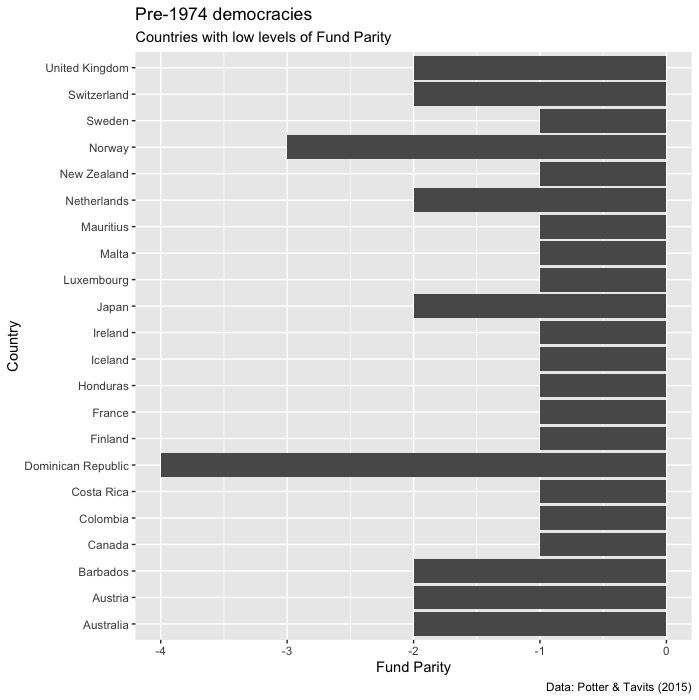
\includegraphics[width = \linewidth, height = .89\textheight]{Rplot05.jpeg}
		\end{minipage}
		\begin{minipage}[b]{0.49\linewidth}
			\centering
			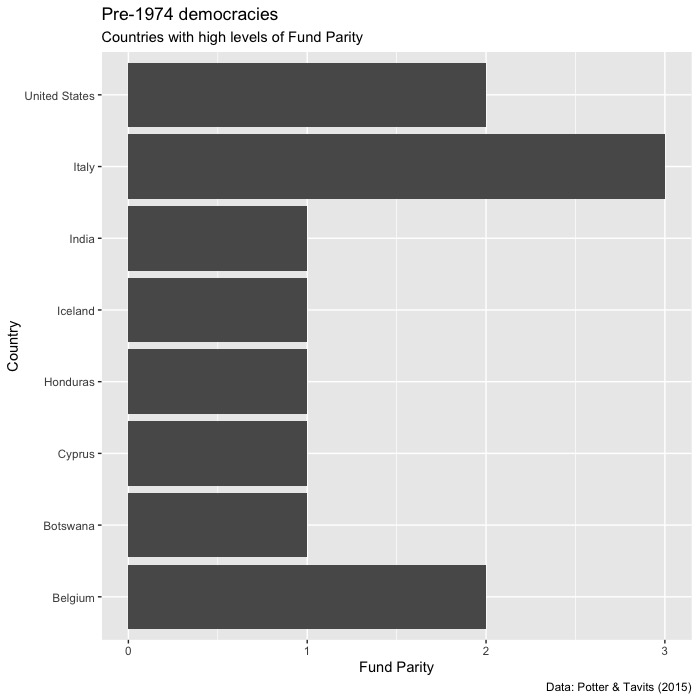
\includegraphics[width = \linewidth, height = .89\textheight]{Rplot06.jpeg}
		\end{minipage}
	\end{figure}
\end{frame}

% GGPLOT OF THE I.V. (Continued) - post 1974 

\begin{frame}
	\frametitle{}
	\begin{figure}
		\begin{minipage}[b]{0.49\linewidth}
		\centering
		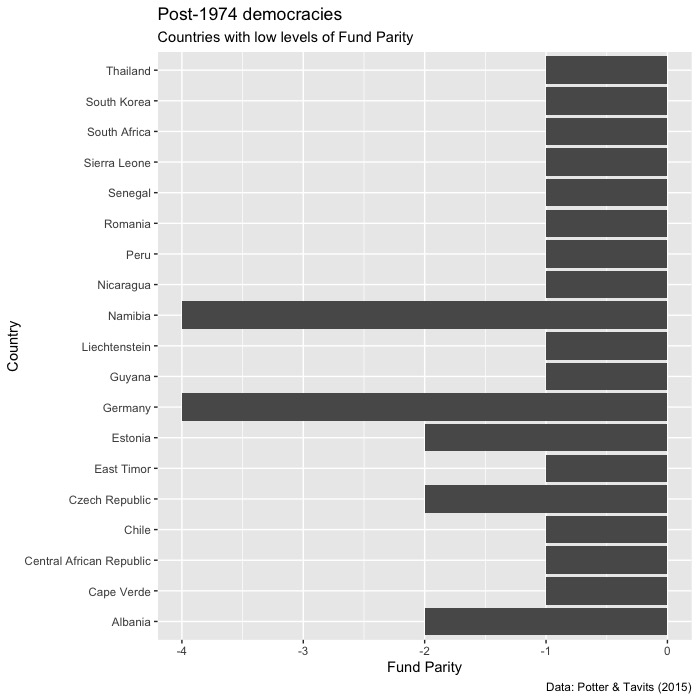
\includegraphics[width = \linewidth, height = .89\textheight]{Rplot04.jpeg}
	\end{minipage}
\begin{minipage}[b]{0.49\linewidth}
	\centering
	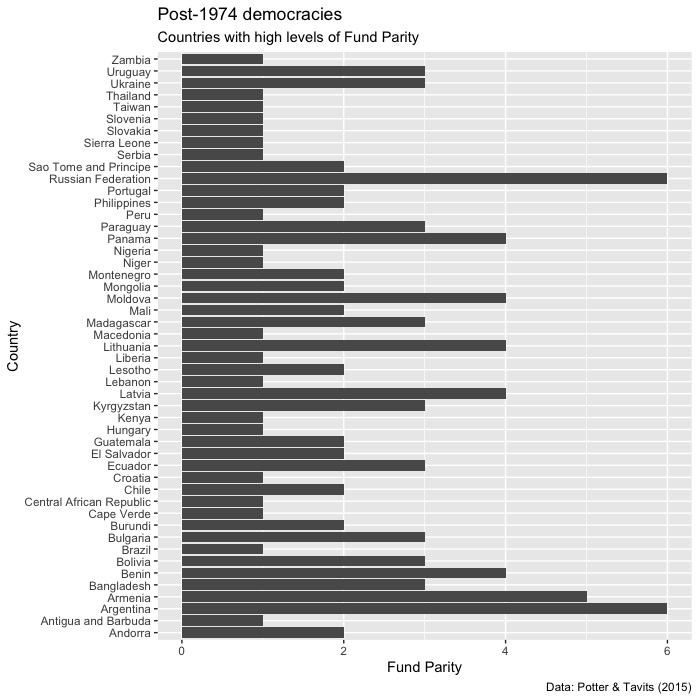
\includegraphics[width = \linewidth, height = .89\textheight]{Rplot03.jpeg}
\end{minipage}
\end{figure}
\end{frame}

	
%% RESEARCH PROPOSAL 

\begin{frame}
	\frametitle{Research Proposal} 
		\textbf{Methodology}
	\begin{itemize}
		\item{Bayesian Analysis} \\~\
	\end{itemize}
\textbf{Hypothesis} 
\begin{itemize}
		\item{Relationship between fund parity and countries GDP}
\end{itemize}
\end{frame}

% Diagnostic

\begin{frame}
	\frametitle{Diagnostic} 
	\begin{itemize}
		\item{Monte Carlo} \\
		\item{Simulate the findings} \\ 
		\item{Use the simulation to re-create the OLS model} \\ 
	\end{itemize}
\end{frame}


\end{document}
